\documentclass[12pt]{ociamthesis}\usepackage[]{graphicx}\usepackage[]{color}
%% maxwidth is the original width if it is less than linewidth
%% otherwise use linewidth (to make sure the graphics do not exceed the margin)
\makeatletter
\def\maxwidth{ %
  \ifdim\Gin@nat@width>\linewidth
    \linewidth
  \else
    \Gin@nat@width
  \fi
}
\makeatother

\definecolor{fgcolor}{rgb}{0.345, 0.345, 0.345}
\newcommand{\hlnum}[1]{\textcolor[rgb]{0.686,0.059,0.569}{#1}}%
\newcommand{\hlstr}[1]{\textcolor[rgb]{0.192,0.494,0.8}{#1}}%
\newcommand{\hlcom}[1]{\textcolor[rgb]{0.678,0.584,0.686}{\textit{#1}}}%
\newcommand{\hlopt}[1]{\textcolor[rgb]{0,0,0}{#1}}%
\newcommand{\hlstd}[1]{\textcolor[rgb]{0.345,0.345,0.345}{#1}}%
\newcommand{\hlkwa}[1]{\textcolor[rgb]{0.161,0.373,0.58}{\textbf{#1}}}%
\newcommand{\hlkwb}[1]{\textcolor[rgb]{0.69,0.353,0.396}{#1}}%
\newcommand{\hlkwc}[1]{\textcolor[rgb]{0.333,0.667,0.333}{#1}}%
\newcommand{\hlkwd}[1]{\textcolor[rgb]{0.737,0.353,0.396}{\textbf{#1}}}%
\let\hlipl\hlkwb

\usepackage{framed}
\makeatletter
\newenvironment{kframe}{%
 \def\at@end@of@kframe{}%
 \ifinner\ifhmode%
  \def\at@end@of@kframe{\end{minipage}}%
  \begin{minipage}{\columnwidth}%
 \fi\fi%
 \def\FrameCommand##1{\hskip\@totalleftmargin \hskip-\fboxsep
 \colorbox{shadecolor}{##1}\hskip-\fboxsep
     % There is no \\@totalrightmargin, so:
     \hskip-\linewidth \hskip-\@totalleftmargin \hskip\columnwidth}%
 \MakeFramed {\advance\hsize-\width
   \@totalleftmargin\z@ \linewidth\hsize
   \@setminipage}}%
 {\par\unskip\endMakeFramed%
 \at@end@of@kframe}
\makeatother

\definecolor{shadecolor}{rgb}{.97, .97, .97}
\definecolor{messagecolor}{rgb}{0, 0, 0}
\definecolor{warningcolor}{rgb}{1, 0, 1}
\definecolor{errorcolor}{rgb}{1, 0, 0}
\newenvironment{knitrout}{}{} % an empty environment to be redefined in TeX

\usepackage{alltt}  % default square logo 
%\documentclass[12pt,beltcrest]{ociamthesis} % use old belt crest logo
%\documentclass[12pt,shieldcrest]{ociamthesis} % use older shield crest logo

%load any additional packages
\usepackage{amssymb}
\usepackage[english]{babel}
\usepackage{graphicx}
\graphicspath{{figure/}}
\usepackage{amsmath}
\usepackage{listings}
\usepackage{enumitem}
\newlist{todolist}{itemize}{2}
\setlist[todolist]{label=$\square$}
\usepackage{pifont}
\usepackage{url}
\usepackage{lipsum}
\usepackage{array}
\usepackage{float}
\usepackage[%
  backend=bibtex      % biber or bibtex
 ,style=numeric-comp    % Alphabeticalsch
 %,style=numeric-comp  % numerical-compressed
 ,sorting=none        % no sorting
 ,sortcites=true      % some other example options ...
 ,block=none
 ,indexing=false
 ,citereset=none
 ,isbn=true
 ,url=true
 ,doi=true            % prints doi
 ,natbib=true         % if you need natbib functions
]{biblatex}

\addbibresource{refs.bib} %Imports bibliography file

\newcommand{\cdifficile}{Clostridium \textit{difficile}}
\newcommand{\cdiff}{C. \textit{diff}}
\newcommand{\cmark}{\ding{51}}%
\newcommand{\xmark}{\ding{55}}%
\newcommand{\done}{\rlap{$\square$}{\raisebox{2pt}{\large\hspace{1pt}\cmark}}%
\hspace{-2.5pt}}
\newcommand{\wontfix}{\rlap{$\square$}{\large\hspace{1pt}\xmark}}
% Confidence interval
\newcommand{\ci}[3]{#1 (95\% CI, #2-#3)}
% Confidence interval with percent
\newcommand{\cip}[3]{#1\% (95\% CI, #2\%-#3\%)}

%input macros (i.e. write your own macros file called mymacros.tex 
%and uncomment the next line)
%\include{mymacros}

%note \\[1ex] is a line break in the title
\title{A Longitudinal Study of the Effect of Renal Failure on Readmission Rates of Patients with \textit{Clostridium Difficile}}

\author{Brian Detweiler}
\college{College of Arts and Sciences}  %your college

%\renewcommand{\submittedtext}{change the default text here if needed}
\degree{Master of Science}     %the degree
\degreedate{May 13, 2017}         %the degree date

%end the preamble and start the document
\IfFileExists{upquote.sty}{\usepackage{upquote}}{}
\begin{document}

%this baselineskip gives sufficient line spacing for an examiner to easily
%markup the thesis with comments
\baselineskip=18pt plus1pt

%set the number of sectioning levels that get number and appear in the contents
\setcounter{secnumdepth}{3}
\setcounter{tocdepth}{3}


\maketitle                  % create a title page from the preamble info

% include a dedication.Rnw file
%<<dedication, child='dedication.Rnw'>>=
%@
 
% include an acknowledgements.Rnw file%
%<<acknowledgements, child='acknowledgements.Rnw'>>=
%@

% include the abstract

\begin{abstract}
\cdifficile Infection (\cdiff, or simply CDI) 
is a highly contagious endospore forming bacterium that is transferred
through physical contact with an infected surface. Symptoms range from diarrhea to
life-threatening colitis and is most commonly acquired in a hospital setting where
antimicrobials have been administered. Increased mortality in
CDI patients with renal failure comorbidities has appeared in the literature as early as 1998 \cite{Cunney1998}.
In this study, we use the \textit{Nationwide Readmissions Database} to assess the risk of 
30, 60, and 90 day readmissions in patients with comorbid 
CDI and renal failure conditions. We also discuss general CDI trends from 2001-2014, using the 
\textit{Nationwide Inpatient Sample}. 
\end{abstract}

\begin{romanpages}          % start roman page numbering
\tableofcontents            % generate and include a table of contents
\listoffigures              % generate and include a list of figures
\listoftables
\end{romanpages}            % end roman page numbering


















%now include the files of latex for each of the chapters etc

\chapter{Introduction}

\section{Overview of \cdifficile}

\cdifficile Infection - also referred to by its shortened name, \cdiff, or simply CDI -
has been an increasing concern in the last two decades among healthcare providers. 
The organism itself is a resilliant endospore-forming bacterium, resistant to heat, acid, and antibiotics,
and can survive on surfaces for up to 5 months, if proper sanitation is not carried out. \cite{Gerding2008}

In past years, the most common CDI cases occurred in elderly patients, 65 years or older,
who were on admitted as an inpatients in a hospital or nursing home setting, and given antimicrobial therapy.
In fact, it has become the most frequent nosocomial (hospital-acquired) disease, surpassing
methicillin-resistant Staphylococcus aureus (MRSA). \cite{Gupta2014}

Antimicrobials deplete the healthy gut flora the intestines which protect against harmful organisms like \cdiff. \cite{Lamont2017}

Adding to the complexity of the situation, CDI carriers can remain asymptomatic, making them stealth transporters
and allowing the disease to propegate undetected until it is too late. 

In 2013, the CDC estimated that around 250,000 Americans contracted \cdiff in a single year, causing 14,000 deaths.
That estimate was later updated to half a million in 2015, causing 15,000 deaths. \cite{CDC2018}
\cite{CDC2015} 
Another study puts that number even higher, at 29,000 deaths in 2011. 

CDI is also costly. The CDC estimates that in 2008, it cost acute healthcare facilities alone more than \$4.8 billion.
The mean cost of an incident of CDI was found to be \$11,498 (inflation adjusted to 2008 dollars)
and as high as \$15,397 when CDI was hospital acquired. \cite{Dubberke2012}


\section{Overview of Renal Failure}

While CDI is a singular diagnosis category, renal failure falls into one of two umbrella categories, acute kidney injury (AKI), 
and chronic kidney disease (CKD). AKI is further broken into subcategories. Acute tubular necrosis is the most common form of AKI.
Other subcategories include renal cortical necrosis, renal medullary necrosis, lesions, and a category for unspecified AKI. 

Chronic kidney disease is broken into categories based on stages that are calculated using one of the estimated Glomerular Filtration Rate
equations. The equations model kidney health as a function of age, sex, race, and blood creatinine, a waste product that is produced from
normal muscle use. 

\subsection{The MDRD Equation vs. the CKD-EPI Equation}

The MDRD equation encodes sex and race (African American or not) and does not rely on height or weight due to using $1.73m^2$ surface area,
the generally accepted mean human adult body surface area. 

\begin{equation} \label{mdrd}
\begin{split}
  GFR  &= 175 \times S_{cr} - 1.154 \times \text{Age}^{-0.203} \times 0.742 \cdot I(\text{F}) \times 1.212 \cdot I(\text{AA}) \\
\end{split}
\end{equation}

The CKD-EPI equation makes use of a 2-slope spline. It was shown to outperform the MDRD, with lower bias and increased precision.  \cite{Levey2009, eGFR2018}

\begin{equation} \label{ckdepi}
\begin{split}
  GFR &= 141 \times min\bigg(\frac{S_{cr}}{\kappa}, 1\bigg)^{\alpha} \times max\bigg(\frac{S_{cr}}{\kappa}, 1\bigg)^{-1.209} \\
      &\times 0.993^{\text{Age}} \times 1.018 \cdot \text{I}(\text{F}) \times 1.159 \cdot \text{I}(\text{AA}) \\
\end{split}
\end{equation}

where:
\begin{itemize}
  \item F is female sex
  \item AA is African American race
  \item I is an indicator function that returns 1 if true, the reciporcal of the preceding term if false (thereby making the preceding term 1)
  \item $S_{cr}$ is serum creatinine in mg/dL
  \item $\kappa$ is 0.7 for females and 0.9 for males
  \item $\alpha$ is -0.329 for females and -0.411 for males
\end{itemize}


\subsection{Classifying Chronic Kidney Disease}

Once the GFR is calculated, patients can be placed into one of five categories. Table \ref{tab:gfr} shows the 
GFR rating along with the stage of CKD and the level of kidney function. \textbf{585} is used in the ICD-9-CM coding system
to indicate CKD. If the level is known, a more specific coding is used. \textbf{585.6} is used for end stage renal disease,
and \textbf{585.9} is used if the level is unspecified.

\begin{table}[]
\centering
\label{my-label}
\begin{tabular}{lllll}
CKD Stage & Description             & GFR        & Kidney Function & ICD-9-CM \\
\hline
1         & Normal function         & 90+        & 90-100\%        & 585.1    \\
2         & Mild loss               & 60-89      & 60-89\%         & 585.2    \\
3         & Mild to severe          & 30-59      & 30-59\%         & 585.3    \\
4         & Severe                  & 15-29      & 15-29\%         & 585.4    \\
5         & Kidney failure          & 15 or less & 15\% or less    & 585.5    \\
\end{tabular}\caption{GFR classifications}\label{tab:gfr}
\end{table}

\subsection{End stage renal disease}

End stage renal disease (ESRD) is diagnosed when CKD reaches its most severe point and dialysis or a kidney transplant is needed to stay alive.
The most common causes of ESRD are diabetes and high blood pressure. Risk of ESRD also increases with age.


\section{Readmissions and the ACA}

A 2014 study done by the Agency for Healthcare Research and Quality (AHRQ) under the Healthcare Cost and Utilization
Project (HCUP) found hospital readmissions accounted for about \$41.3 billion in hospital costs.  \cite{Hines2014}

Under the Readmission Reduction Program, a provision of the Affordable Care Act, 
Hospitals face penalties on Medicare payments if they exceed certain 30-day readmission standards. While the 
American Hospital Association strongly opposes the measure, citing a lack of control over the chain of events
that can lead to readmission \cite{Rice2015, AHA2018}, the Affordable Care Act is still the rule of law, and hospitals must seek
to reduce readmissions in order to avoid penalties.

For this reason, readmission statistics are an important key metric for hospitals interested in optimizing 
their operations. Using large surveys, researchers are able to determine trends and end results, but not necessarily 
causes, of readmissions. Still, high level trends can point healthcare providers in a direction where they can
more efficiently focus their attention. 

\subsection{Readmission measures}

The Centers for Medicare \& Medicaid Services (CMS) sets guidelines that hospitals must follow to avoid penalization on Medicare payments. 
The CMS measures "excess readmissions" as a ratio of predicted-to-expected readmissions and each hospital's relative performance, based on
a 30-day risk standardized measure. All-cause unplanned readmissions to the same or another applicable acute care hospital, 
ocurring within 30 days - for any reason, regardless of principal diagnosis - from the index admission are counted in this measure.
Some planned readmissions are not counted. \cite{HRRP}

For fiscal years 2013 to 2018, the following formula is used to calculate the Payment Readjustment Factor (PRF):

\begin{equation} \label{prf}
\begin{split}
  \text{PRF} &= 1 - min\bigg(0.03, \sum_{dx} \frac{\text{Payment}(dx) \cdot max\big((\text{ERR}(dx) - 1.0), 0\big)}{\text{All payments}}\bigg) \\
\end{split}
\end{equation}
 
Where $dx$ is one of six measure cohorts: 

\begin{itemize}
  \item acute myocardial infarction (AMI)
  \item heart failure (HF)
  \item pneumonia
  \item chronic obstructive pulmonary disease (COPD)
  \item coronary artery bypass graft (CABG) surgeries
  \item elective primary total hip and/or total knee arthroplasty (THA/TKA)
\end{itemize}

ERR is a hospital's performance measure $dx$, and payment refers to base operating DRG payments. \cite{HRRPPaymentAdjustment, Lessa2015}


\section{Overview of the data}

The Agency for Healthcare Research and Quality (AHRQ), under the Department of Health and Human Services (DHHS), sponsors the
Healthcare Cost and Utilization Project (HCUP), a collection of databases including the Nationwide Inpatient Sample (NIS) and
the Nationwide Readmissions Database (NRD). \cite{HCUPOverview}

\subsection{The Nationwide Inpatient Sample (NIS)}

The Agency for Healthcare Research (AHRQ) has been conducting the National (later renamed to "Nationwide") Inpatient
Sample since 1988, as part of the Healthcare Cost and Utilization Project (HCUP). It estimates a weighted 35 million
hospitalizations per calendar year using around 7-8 million unweighted discharges per year. It is the largest database
of its kind in the United States. \cite{NISOverview}

\subsection{The Nationwide Readmissions Database (NRD)}

Similar to the NIS, the NRD tracks hospitalizations. In addition, it tracks patients across admissions, using an ID key,
an admission reference date, and a length of stay for each admission. This allows analysts to track anonymized readmission cases.
The NRD tracks around 14 million unweighted patients, when weighted, estimates about 36 million weighted patients across admissions 
per calendar year. \cite{NRDOverview} 

\subsection{Limitations}

Working on such a rich dataset does not come without limits. Prior to obtaining the NIS or NRD, analysts must take the HCUP
Data Usage Agreement (DUA). At a high level, HCUP requires that researchers protect individual identities. Cell sizes where $n \le 10$ 
may not be reported. Attempting to identify individual patients or health care providers through vulnerability or penetration testing, 
or any other means, is prohibited. Publication of any methodology that could identify individuals is prohibited.

Furthermore, HCUP data may only be used for research, not for commercial or competitive purposes. Institutions may not be contacted
to verify any of the data within the HCUP datasets either. 

For the above reasons, the data may also not be posted online, and anyone wishing to work with or even see the data must take the DUA class and
sign the agreement. \cite{HCUPDUA}

In a couple of recent publications, Khera and Krumholz expanded on these base requirements and offered a checklist \cite{Krumholz2017} 
for analysts to follow as they work with the NIS. In a followup study, they found only 10.5\% (95\% CI, 4.7\%-16.4\%) of published research
projects based on NIS data followed all of the guidelines. \cite{Khera2017}

Listed below are the guidelines from Khera and Krumholz, and notes on how we have conformed to them.


\begin{itemize}
  \item  \textbf{Section A: Research Design}
  \begin{todolist}
  \item[\done] Does the study consider that it can only detect disease conditions, procedures, and diagnostic tests in hospital settings?
  
  \textbf{Yes, we make no assumptions about events occurring outside of the hospital setting.}
  
  \item[\done] Does the study acknowledge that it includes encounters, not individual patients?
  
  \textbf{Yes, all of our assumptions are made upon the basis of inpatient discharges and readmissions, not individuals.}
  
  \item[\done] Does the study avoid diagnosis/procedure-specific volume assessments for units that are not part of the
  sampling frame of the NIS, and are therefore not representatively sampled, including
  
  \begin{itemize}
    \item geographic units, like U.S. states
    \item healthcare facilities (after 2011)
    \item individual healthcare providers?
  \end{itemize} 
          
  \textbf{Yes, we only make assessments at the national level.}
  
  \end{todolist}
  
  \item  \textbf{Section B: Data Interpretation}
  \begin{todolist}
  \item[\done] Does the study attempt to identify disease conditions or procedures of interest using administrative 
  codes or their combinations that have been previously validated?
 
  \textbf{Yes, when checking for renal failure, the comorbidity indicators (\texttt{renlfail, cm\_renlfail}) were used 
  before assessing ICD-9-CM codes.}
  
  \item[\done] Does the study limit its assessments to only in-hospital outcomes, rather than those occurring after discharge?
  
  \textbf{Yes, the only outcome assessments were readmission status and mortality (\texttt{died}), both of which are in-hospital events.}
  
  \item[\done] Does the study distinguish complications from comorbidities or clearly note where it cannot?
  
  \textbf{Yes, renal failure comorbidities were distinguished using the the comorbidity indicators (\texttt{renlfail, cm\_renlfail}). 
  CDI while most often a complication, cannot usually be distinguished between complication and comorbidity however.}
  
  
  \end{todolist}
  
  \item  \textbf{Section C: Data Analysis}
  \begin{todolist}
  \item[\done] Does the study clearly account for the survey design of the NIS and its components -clustering, stratification, and weighting?
 
  \textbf{Yes, the R \texttt{survey} package was used to account for survey design.}
  
  \item[\done] Does the study adequately address changes in data structure over time (for trend analyses)?
  
  \textbf{Yes, since we are only doing national-level assessments, and we are not using ICD-10-CM codes in the 2015 datasets, 
  we don't need to worry about the changes in the survey design.}
  
  \end{todolist}
  
\end{itemize}



\chapter{Methods}




All analyses were done in R version 3.4.3 (2017-11-30) on an x86\_64-pc-linux-gnu (64-bit) 
running Ubuntu 16.04.4 LTS. 
Complex survey designs of the NIS and NRD  were accounted for using the \texttt{survey} package, version 
3.33-2. \cite{Lumley2018} Data were stored and retrieved in
MonetDB using MonetDBLite version 0.5.1.
\cite{Muehleisen2018}

\section{Data source}

Years 2001-2014 of the NIS, as well as years 2010-2014 of the NRD were provided courtesy of Creighton University
School of Medicine. Both datasets originate in comma-separated variables (CSV) format. 

The NIS covers between 7-8 million unweighted patients per calendar year, resulting in file sizes around 3 GB on average,
totaling around 43 GB of raw ASCII text.

\begin{lstlisting}[language=Bash]
  $ l -ha NIS* | awk '{print $5, $9}'
  2.7G NIS2001.csv                                                          
  2.9G NIS2002.csv                                                          
  3.0G NIS2003.csv                                                          
  3.1G NIS2004.csv                                                          
  3.1G NIS2005.csv                                                          
  3.1G NIS2006.csv                                                          
  3.4G NIS2007.csv                                                          
  3.4G NIS2008.csv                                                          
  3.5G NIS2009.csv
  3.6G NIS2010.csv
  3.7G NIS2011.csv
  2.6G NIS2012.csv
  2.6G NIS2013.csv
  2.8G NIS2014.csv
\end{lstlisting}

The NRD is normalized into 4 different files, 3 discharge-level files and a hospital-level file.

The \texttt{Core} file contains data elements necessary for readmission analysis. The \texttt{Severity} files
contain data related to the severity of the patients' conditions, including, for our purposes, comorbidity flags.
The \texttt{DX\_PR} file (diagnoses and procedures) file contains ICD-9-CM codes and other fields related to
diagnoses and procedures. Finally, the hospital file contains information on the hospital characteristics.

The NRD is a record of around 14 million unweighted admissions per calendar year with identifiers that allow analysts 
to track readmissions from a particular index event.

\begin{lstlisting}[language=Bash]
  $ l -ha NRD*/*.CSV | awk '{print $5, $9}' | sed -e 's/ /\t/'
  5.0G    NRD2010/NRD_2010_Core_V2.CSV
  3.4G    NRD2010/NRD_2010_DX_PR_GRPS_V2.CSV
  88K     NRD2010/NRD_2010_Hospital_V2.CSV
  1.2G    NRD2010/NRD_2010_Severity_V2.CSV
  5.1G    NRD2011/NRD_2011_Core_V2.CSV
  3.4G    NRD2011/NRD_2011_DX_PR_GRPS_V2.CSV
  87K     NRD2011/NRD_2011_Hospital_V2.CSV
  1.2G    NRD2011/NRD_2011_Severity_V2.CSV
  4.9G    NRD2012/NRD_2012_Core_V2.CSV
  3.3G    NRD2012/NRD_2012_DX_PR_GRPS_V2.CSV
  82K     NRD2012/NRD_2012_Hospital_V2.CSV
  1.1G    NRD2012/NRD_2012_Severity_V2.CSV
  5.2G    NRD2013/NRD_2013_Core.CSV
  3.4G    NRD2013/NRD_2013_DX_PR_GRPS.CSV
  92K     NRD2013/NRD_2013_Hospital.CSV
  1.1G    NRD2013/NRD_2013_Severity.CSV
  6.6G    NRD2014/NRD_2014_Core.CSV
  4.1G    NRD2014/NRD_2014_DX_PR_GRPS.CSV
  98K     NRD2014/NRD_2014_Hospital.CSV
  1.2G    NRD2014/NRD_2014_Severity.CSV
\end{lstlisting}

This totals to over 50 GB of raw ASCII text. 

\subsection{Persistence}

There are numerous ways to handle a dataset of this size. If we know exactly what unique codes we want,
we could simply \texttt{grep} for them. However, this isn't scalable and we would not be able to calculate
population proportions.

For this project, we imported the data into MonetDBLite, an in-process version of MonetDB. 
We chose MonetDB, because it fits well in the academic space, being open source with strong R 
integration and good community support.
It also fits well in the data warehousing space, being a pioneer in column-store technologies. 

Column-store databases partition each column as an array, making data retrieval extremely fast when
only a subset of the columns need to be loaded into memory. \cite{MonetDB}

\subsection{Diagnosis and procedure codes}

The International Classification of Diseases, Ninth Revision, Clinical Modification (ICD-9-CM) is based on the World Health Organization's Ninth Revision,
International Classification of Diseases (ICD-9). It is the coding standard for diseases and procedures used in the NIS and NRD up to October, 2015, when
HCUP upgraded to ICD-10-CM. 

Although we had access to the 2015 NRD data, it was not used due to the added complexity of accounting for ICD-10-CM changes, as well as not having 2015
data for NIS, which would have caused inconsistencies in trend analysis. 

With the acknowledgement that ICD-9-CM codes are not perfect \cite{Uchiyama2015}, they are still the best thing we have for longitudinal 
epidemiological studies on a large scale. 

All diagnosis fields, \texttt{dx1, dx2,} $\hdots$ \texttt{dx30} were queried for code \textbf{00845} (\textit{Intestinal infection due to Clostridium difficile}). 
The decision not to look exclusively at \texttt{dx1}, the principal diagnosis, was deliberate, due to the nature of \cdiff. Patients rarely contract CDI
independently. It is typically contracted while in a hospital setting while being treated for a separate disease. 

To complicate matters, ICD-9-CM codings are not an exact science, and are often done based on cost and seriousness of comorbid conditions. Coders must use
their judgement for determining a principal diagnosis when comorbid conditions are present. \cite{Avery2011} For this reason, we simply simply queried for
the presence of the condition on any diagnosis field. 

The same was done for renal failure codes.

\begin{table}[]
\centering
\caption{ICD-9-CM renal failure codes}
\label{icd9renal}
\begin{tabular}{ll}
Code  & Description          \\
\hline
584   & Acute kidney failure \\
584.5 &	Acute kidney failure with lesion of tubular necrosis convert \\
584.6 &	Acute kidney failure with lesion of renal cortical necrosis convert \\
584.7 &	Acute kidney failure with lesion of renal medullary [papillary] necrosis \\
584.8 &	Acute kidney failure with lesion of with other specified pathological lesion in kidney \\
584.9 &	Acute kidney failure, unspecified \\
585   & Chronic kidney disease (ckd) \\
585.1 &	Chronic kidney disease, Stage I \\
585.2 &	Chronic kidney disease, Stage II (mild) \\
585.3 &	Chronic kidney disease, Stage III (moderate) \\
585.4 &	Chronic kidney disease, Stage IV (severe) \\
585.5 &	Chronic kidney disease, Stage V (mild) \\
585.6 &	End stage renal disease \\
585.9 &	Chronic kidney disease, unspecified \\
586   &	Renal failure, unspecified \\
\end{tabular}
\end{table}

For trend analysis, the CDI and renal failure selections were joined. This provided full samples of
CDI and renal patients, as well as patients with both.


\subsection{Determining index admissions and radmissions}

Unlike the NIS, the NRD allows tracking patients across hospital visits within a given calendar year.
The field \texttt{nrd\_visitlink} provides a key that identifies a single patient across multiple visits.
To determine temporality, a length of stay field (\texttt{los}) is provided for each visit, as well as
a reference date, \texttt{nrd\_daystoevent}. To ensure anonymity, a randomly selected date is chosen for 
each patient. \texttt{nrd\_daystoevent} then references the random date and lists the days from the epoch date.
This way, no precise date can be determined, thereby protecting patient privacy, while providing the researcher
with the data he or she needs. 

The NRD leaves readmission determination up to the analyst. First an index event must be chosen. 
We selected all cases of CDI (ICD-9-CM code \textbf{00845}) and retrieved all unique \texttt{nrd\_visitlink}
identifiers. Then a second query was performed retrieving all events for the \texttt{nrd\_visitlink} identifiers.

We then grouped the cases first by \texttt{nrd\_visitlink}, then chronologically. Then, we scanned for the first
occurrence of a CDI event (ICDM-9-CM code \textbf{00845}) and marked it as the index event. All information from
the index event was stored in a "patient profile" object. The remaining patient admissions, if any, were scanned.
If the event contained a CDI identifier and fell within the given readmission day window (30, 60, and 90 days, separately),
the event was considered a readmission and the number of readmissions were stored. If the patient died on a readmission,
that was also stored. If the secondary event fell outside of the readmission window, it was considered another index event, 
and the process started over.

The following additional rules were applied for determining index events for \textit{d}-day readmissons, where $d = \{30, 60, 90\}$:

\begin{enumerate}
    \item For years 2010-2014: ($1 \le \text{DMONTH} \le 12 - ceil(d/30)$)
    
    We needed to cut off index events with enough time to determine if there was a readmission, since only calendar years can be analyzed.
    
    \item $\text{DIED} \ne 0$
    
    A death on index does not allow for readmission.
    
    \item $\text{LOS} > 0$
    
    A length of stay equal to zero represents transfers and same-day stays that were combined which represents a more complex type of care. \cite{NRDIntroduction2013}
    
    \item $AGE > 0$
  
    About 70\% of infants under one year of age carry \cdiff without showing signs or symptoms. \cite{Lamont2017} 
    
\end{enumerate}



\begin{figure}[h]
\centering
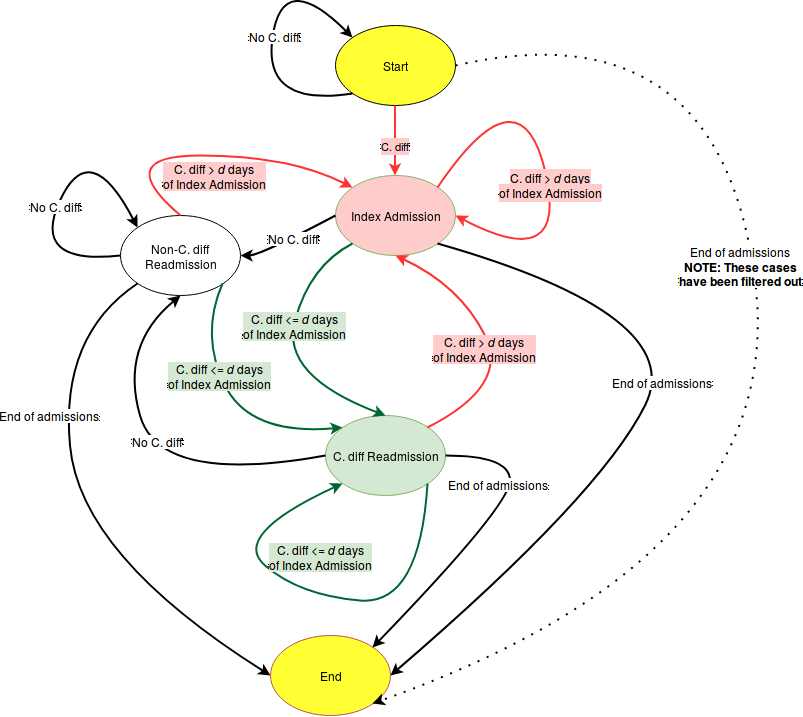
\includegraphics[scale=0.5]{readmission-state-diagram.png} 
\label{fig:readmission-state-diagram} 
\caption{State diagram for determining what constitutes an index admission and a subsequent readmission.
Additional rules include cutting off index events by October, November, or December, depending on whether we are looking for 90, 60, 30 day readmissions, respectively;
filtering out deaths on index events;
lengths of stay that included transfers and same-day stays;
and infants less than 1 year of age, where \cdiff is common but shows no symptoms.}
\end{figure}


\subsection{Choosing features}

To determine renal failure comorbidities, the \texttt{cm\_renlfail} flag was first used, and then more specific ICD-9-CM codes were identified. Acute kidney failure, 
or acute kidney injury (AKI) were grouped by all sub-category codes into a single AKI category. This included codes \textbf{584}, \textbf{584.5}, \textbf{584.6}, \textbf{584.7}, 
\textbf{584.8}, and \textbf{584.9}. 

Chronic kidney disease (CKD) stages were individually analyzed, but unspecified or unknown CKD cases were grouped, (ICD-9-CM codes \textbf{585} and \textbf{585.9}). 

Additionally, we considered hospital characteristics as independent factors, including hospital control (Government, nonfederal; Private, non-profit; Private, invest-own), 
urban/rural designation (9 categories from smallest to largest), teaching designation, and bedsize. 

Hospital urban/rural designations contained 9 categories 1 being the largest and 9 being the smallest. These were reversed in order to have a meaningful effect in the regression.

Sex was also included in the regression.

Patients' age is included in the eGFR formula, and as such, would be a confounding variable, so it was not included in the regression.

\section{Statistical analysis}

Descriptive and inferrential statistics were done using the NIS and NRD complex survey design, 
supplying \texttt{hospid} as the clusters, \texttt{nis\_stratum} as the strata, and \texttt{discwt} as the weighting. 
Lonely primary sampling units (PSU) - in our case, hospitals - were excluded using \texttt{options(survey.lonely.psu="remove")}. \cite{LonelyPSUs}

The primary readmission analysis was done with multivariable logistic regression to determine the effect of the covariates and confounding variables
on the likelihood of being readmitted with CDI under the three readmission windows, 30, 60, and 90 days. 

The model was fitted independently on each year's data. 
We could have included the years as independent variables and attempted to fit the entire dataset, but we chose not to. The primary reason being, the dataset is very large,
so a single all-year fit was somewhat impractical due to hardware resource limitations. More academically, however, we are able to capture more nuance in modelling individual
years, given each year is a separate independent data set, and medical trends do change over time. Fitting 5 years of data all at once, is likely to miss smaller subtleties, 
such as increases or decreases in a particular coefficient over time. 

Variance estimation was done using Jackknife Repeated Replication (JRR), specifically the JKn approach. Replication methods have shown better
precision and reduced bias compared to Taylor Series Linearization. \cite{Chowdhury2013, Smith2000}

All charts were done with the \texttt{ggplot2} package. 

\chapter{Results}


\section{Trends}

\begin{knitrout}
\definecolor{shadecolor}{rgb}{0.969, 0.969, 0.969}\color{fgcolor}\begin{figure}

{\centering \includegraphics[width=\maxwidth]{figure/fig:disease_trends_cdi-1} 

}

\caption[CDI trends show a somewhat linearly increasing trend]{CDI trends show a somewhat linearly increasing trend. If we extrapolate to 2018, we have a rough idea of the proportion of the inpatient population we can expect to be diagnosed with CDI.}\label{fig:fig:disease_trends_cdi}
\end{figure}


\end{knitrout}
\label{fig:disease_trends_cdi}

Over the 14 year period, from 2010 - 2014, the proportion of inpatients with CDI increased from 
\cip{0.003998292}{0.003773284}{0.004236661} in 2001, roughly 
\ci{141,540}{133,574}{149,978} people, to
\cip{0.01023635}{0.01004522}{0.01043108} in 2014, or
\ci{362,367}{355,601}{369,260} people - 
a difference of about 0.006238055\%, or 220,827 people. 



\begin{knitrout}
\definecolor{shadecolor}{rgb}{0.969, 0.969, 0.969}\color{fgcolor}\begin{figure}

{\centering \includegraphics[width=\maxwidth]{figure/fig:disease_trends_cdi_renal-1} 

}

\caption[Comparitively, CDI occurrences are not increasing as rapidly as renal diseases]{Comparitively, CDI occurrences are not increasing as rapidly as renal diseases. The sharp spikes from 2004-2006 were likely due to ICD-9-CM coding requirements implemented in October of 2005.}\label{fig:fig:disease_trends_cdi_renal}
\end{figure}


\end{knitrout}
\label{fig:disease_trends_cdi_renal}



\begin{knitrout}
\definecolor{shadecolor}{rgb}{0.969, 0.969, 0.969}\color{fgcolor}\begin{figure}

{\centering \includegraphics[width=\maxwidth]{figure/disease_trends_esrd-1} 

}

\caption[Age distribution for ESRD has remained consistent since ICD-9-CM coding standards changed in October, 2005]{Age distribution for ESRD has remained consistent since ICD-9-CM coding standards changed in October, 2005.}\label{fig:disease_trends_esrd}
\end{figure}


\end{knitrout}

\label{fig:disease_trends_esrd}

In Figures  \ref{fig:age_distribution_over_time} and \ref{fig:age_trends}, we can see the median age for inpatient CDI has been lowering over the years.


\begin{knitrout}
\definecolor{shadecolor}{rgb}{0.969, 0.969, 0.969}\color{fgcolor}\begin{figure}

{\centering \includegraphics[width=\maxwidth]{figure/age_trends-1} 

}

\caption[C]{C. 	extit{diff} is trending into younger generations in recent years.}\label{fig:age_trends}
\end{figure}


\end{knitrout}
\label{fig:age_distribution_over_time}

\begin{knitrout}
\definecolor{shadecolor}{rgb}{0.969, 0.969, 0.969}\color{fgcolor}\begin{figure}

{\centering \includegraphics[width=\maxwidth]{figure/cdi_age_ts-1} 

}

\caption[All age groups below 75 show a steady increase in CDI infections]{All age groups below 75 show a steady increase in CDI infections. 75 and older are down from their peaks in the mid 2000s.}\label{fig:cdi_age_ts}
\end{figure}


\end{knitrout}
\label{fig:cdi_age_ts}

\begin{knitrout}
\definecolor{shadecolor}{rgb}{0.969, 0.969, 0.969}\color{fgcolor}\begin{figure}

{\centering \includegraphics[width=\maxwidth]{figure/fig:cdi_males_females-1} 

}

\caption[Females are almost 1.4 times as likely to contract CDI than males]{Females are almost 1.4 times as likely to contract CDI than males.}\label{fig:fig:cdi_males_females}
\end{figure}


\end{knitrout}
\label{fig:cdi_males_vs_females}


\begin{knitrout}
\definecolor{shadecolor}{rgb}{0.969, 0.969, 0.969}\color{fgcolor}\begin{figure}

{\centering \includegraphics[width=\maxwidth]{figure/fig:age_quantile_trends-1} 

}

\caption[The median age for inpatient CDI admissions has been sharply declined since 2006]{The median age for inpatient CDI admissions has been sharply declined since 2006. The vertical bars indicate a 95\% confidence interaval.}\label{fig:fig:age_quantile_trends}
\end{figure}


\end{knitrout}

\label{fig:age_trends}



\section{Readmission risk modeling}








\begin{knitrout}
\definecolor{shadecolor}{rgb}{0.969, 0.969, 0.969}\color{fgcolor}\begin{figure}

{\centering \includegraphics[width=\maxwidth]{figure/fig:30_day_readmission_model-1} 

}

\caption[Coefficient estimates for the 30-day readmission model]{Coefficient estimates for the 30-day readmission model. Here, we only show coefficients that were statistically significant across all years. ESRD is highly significant and a strong predictor of readmission.}\label{fig:fig:30_day_readmission_model}
\end{figure}


\end{knitrout}

\begin{knitrout}
\definecolor{shadecolor}{rgb}{0.969, 0.969, 0.969}\color{fgcolor}\begin{figure}

{\centering \includegraphics[width=\maxwidth]{figure/fig:60_day_readmission_model-1} 

}

\caption[Coefficient estimates for the 60-day readmission model]{Coefficient estimates for the 60-day readmission model. Here, we only show coefficients that were statistically significant across all years. ESRD is highly significant and a strong predictor of readmission.}\label{fig:fig:60_day_readmission_model}
\end{figure}


\end{knitrout}


\begin{knitrout}
\definecolor{shadecolor}{rgb}{0.969, 0.969, 0.969}\color{fgcolor}\begin{figure}

{\centering \includegraphics[width=\maxwidth]{figure/fig:90_day_readmission_model-1} 

}

\caption[Coefficient estimates for the 90-day readmission model]{Coefficient estimates for the 90-day readmission model. Here, we only show coefficients that were statistically significant across all years. ESRD is highly significant and a strong predictor of readmission.}\label{fig:fig:90_day_readmission_model}
\end{figure}


\end{knitrout}


%Proportion of ESRD and CDI that were readmitted


\chapter{Discussion}

\section{Trends in CDI}


\subsection{Increasing infection rates}

\cdiff has been on the rise since the first reported major outbreak of ribotype 027, a hypervirulent strain, in 2004 \cite{Pepin2004}. 
Figure \ref{fig:disease_trends_cdi} shows the trend for CDI using the data from 2001-2014, extrapolated through 2018. 
Over 1\% of the inpatient population in 2014 was diagnosed with CDI. If this trend continues linearly, we can expect that number
to increase to nearly 1.2\% by 2018. 

While the CDC found that around half a million people contracted CDI in 2015, about 150,000 of those were not documented in 
inpatient records, making their inpatient estimate around 350,000. \cite{CDC2018} This is somewhat consistent with our CDI linear model in 
Figure \ref{fig:disease_trends_cdi}, which estimates about \ci{391,293.4}{381,061.4}{401,802.9} people in 2015,
without having the data.

Using this model, we can expect CDI infections to increase to \ci{437,605.1}{427,984.2}{447,380.8} hospital inpatients in 2018, and
\ci{468,479.6}{459,266.1}{477,766.1} in 2020, if the trend continues.

This proportion pales in comparison to renal failure, however, which has also been on the rise, with nearly 10\% of patients coded with
some form of acute kidney injury (ICD-9-CM codes \textbf{584}, and \textbf{584.5}-\textbf{584.9}) or chronic kidney disease 
(ICD-9-CM codes \textbf{585} and \textbf{585.1}-\textbf{585.5}, as well as \textbf{585.9}) in 2014. AKI has risen 
by 0.6189396\% per year on average.

While renal failure is a broad general category, even more specific codings, including the most serious, 
End-Stage Renal Disease, showed much higher inpatient rates than CDI. 
This suggests that CDI is not yet a national epidemic. The trend should continue to be
monitored, however, for drastic increases. If data for future years show the process breaking the previously linear trend, it could be an indication
that something has changed, such as a mutation in the bacterium. Conversely, if infections make a downward turn, research should be done
to determine what methods have been effective in fighting the disease.


\subsection{Infections at a younger age}
We showed a trend in CDI moving into younger age groups. This is consistent with findings by Gupta and Khanna \cite{Gupta2014}. 


Increased age as a risk factor may be confounded by increased risk of other acquired comorbidities such as renal failure. 
\cite{Krapohl2013, Masgala2014}
%has  the elderly, and that continues to be the case today. Caroll and Bartlett \cite{Carroll2011}


Figure \ref{fig:age_distribution_over_time} shows the distribution of \cdiff patients by age for all data from 2001-2014. 

%\cite{Masgala2014}

In 2001, the median age for CDI was 73 (95\% CI, 72-74). In 2014, it had dropped to 68 (95\% CI, 68-69). 

\section{Trends in renal failure}

%\ref{fig:disease_trends_cdi_renal}

The distribution of ESRD has remained consistent since the coding changes in 2005. 
\label{fig:disease_trends_esrd}


\section{Renal failure as a CDI readmission risk factor}

In their 2015 meta-analysis, Phatharacharukul, et. al. found the pooled relative risk of \cdiff-associated diarrhea (CDAD)
in patients with CKD were \ci{1.95}{1.81}{2.10} and \ci{2.63}{2.04}{3.38}, in ESRD patients. \cite{Phatharacharukul2015}
Recurrent CDAD is the primary reason for CDI readmissions.

\chapter{Conclusion and future work}



\section{Future work}

Due to time constraints, we were unable to explore some of the larger questions that arose
from this study. Is the trend in CDI expanding into younger members of the population due
to community-acquired CDI, as shown by Gupta and Khanna? \cite{Gupta2014} Are antibiotics
still being used liberally, causing \cdiff to spread into a broader population? More 
work needs to be done to investigate these trends.


On average, females were 1.397 times as likely to contract CDI. We did not investigate the
reasons for this. One possible contributing factor was that women giving birth may be more susceptible to CDI, but 
verification of this line of thinking is left to future work.

Another topic we were unable to cover was mortality. If ESRD patients contracted CDI, what is their mortality rate?
Findings at the National Kidney Foundation showed mortality to be at 3.8\% among patients with ESRD, compared to
1.46\% for CDI patients without ESRD. \cite{Susman2013} 

These findings should be verified and updated with newer data. 

%now enable appendix numbering format and include any appendices
%\appendix
%<<appendix1, child='appendix1.Rnw'>>=
%@
%<<appendix2, child='appendix2.Rnw'>>=
%@

%next line adds the Bibliography to the contents page
%\addcontentsline{toc}{chapter}{Bibliography}
%uncomment next line to change bibliography name to references
%\renewcommand{\bibname}{References}
%\bibliography{refs}        %use a bibtex bibliography file refs.bib
% \bibliographystyle{plain}  %use the plain bibliography style
% \bibliographystyle{apalike}
\renewcommand{\bibname}{References}
\printbibliography
%Sets the bibliography style to UNSRT and imports the 
%bibliography file "samples.bib".
\end{document}
